% Printed 282; principal PDF 289; Google PDF 293.
\par\clearpage
\noindent\makebox[0pt][l]{\fontsize{13}{16}\selectfont 282}\hfill{\small\textbf{CORRESPONDENCE.}}\hfill\null\par\medskip

\noindent larly what you would like explained. For now I shall only point out that there are two main steps in forming it.

I.\quad Form a table derived \textls[120]{solely} from the measurements at the site and therefore still unoriented.

II.\quad Orient the table by adding a constant. For convenience I like to arrange the first table so that its orientation is already very close.

The first table need only include the directions based on angular measurements that provide some check on one another, together with any of the other directions that may be needed to obtain the absolute orientation. In the present case, the former are [the directions]
\[
\GaussRightBrace{
\begin{array}{@{}r@{\enspace}l@{}}
 1&\text{Neuenfelde}\\
 2&\text{Altenwerder}\\
 3&\text{Altona, heliotrope}\\
 4&\text{Hamburg}\\
 5&\text{Wilhelmsburg}
\end{array}
}\quad\odot
\]
and the latter are [the directions to] the stake, the meridian stake, and perhaps Rönneberg. I would also have included Harburg among the latter if it had been sighted by repetition.

All the measurements relating to the points \(\odot\) are as follows*)
\[
\GaussRightBrace{
\begin{array}{@{}r@{\quad}r@{\qquad}r@{\;}r@{\;}r@{}}
 1.2&5&41^\circ&4'&39''{,}700\\
 1.3&4&45&11&31{,}400\\
 1.4&4&54&45&31{,}562\\
 1.5&5&85&36&40{,}200\\
 2.3&1&4&6&50{,}750\\
 2.5&10&44&32&2{,}275\\
 3.4&28&9&34&1{,}973\\
 3.5&2&40&25&10{,}000\\
 4.5&20&30&51&9{,}255
\end{array}
}\quad\mathrm{A}
\]

\par\smallskip\noindent\rule{4cm}{.4pt}\par
{\footnotesize\noindent\hspace*{\parindent}*) I took the means somewhat differently from Mr.~\textsc{Peters} in some cases.\par}

% Printed 283; principal PDF 290; Google PDF 294.
\par\clearpage
\noindent\null\hfill{\small\textbf{STATION ADJUSTMENTS.}}\hfill\makebox[0pt][r]{\fontsize{13}{16}\selectfont 283}\par\medskip

To obtain Table I for the points \(\odot\), we must first form another, approximate table in which the measurements A have \textls[120]{not yet} been adjusted. To give it at least an approximate orientation, I note that my earlier table for Altona contains the following.
\[
\begin{array}{@{}l@{\;}r@{\;}r@{\;}l@{}}
 \text{\hbox to 8.7em{Harburg\hfil.\hfil.\hfil.\hfil.\hfil.\hfil.\hfil.\hfil.\hfil.}}&344^\circ&52'&54''{,}294\\
 \text{\hbox to 8.7em{Meridian stake\hfil.\hfil.\hfil.\hfil.}}&359&59&56{,}741.
\end{array}
\]

We therefore obtain Vahrendorf as follows.
\[
\begin{array}{@{}l@{\quad}r@{\quad}l@{}}
 \text{from Harburg}&
 \GaussOldenburgLeftBrace{\begin{array}{@{}r@{\;}r@{\;}r@{}}344^\circ&52'&54''{,}294\\28&41&26{,}413\end{array}}&\\[3.5pt]
 \cline{2-2}
 &13\quad34\quad20{,}707&
 \begin{array}[t]{@{}c@{}}\text{15 obs., to which I assign}\\\text{only half weight.}\end{array}\\[5pt]
 \text{from meridian stake}&
 \GaussOldenburgLeftBrace{\begin{array}{@{}r@{\;}r@{\;}r@{}}359&59&56{,}741\\13&34&23{,}400\end{array}}&\\[3.5pt]
 \cline{2-2}
 &13\quad34\quad20{,}141&\text{43 obs.}\\
 \cline{2-2}
 &13^\circ\;34'\;20''{,}225&\text{Mean.}
\end{array}
\]

From the Vahrendorf \textls[120]{stake}, then, the azimuth of Altona would be \(193^\circ\,34'\,20''{,}225\) if the Earth were a plane. Its curvature requires a small reduction, which can be computed only once the position of Vahrendorf is known. There is also the centering correction to the observation site, which likewise cannot yet be computed, though it is negative.

(I inadvertently wrote [positive] here and chose the first number accordingly. This makes no difference at all in Table I, which contained only the relative positions. It is convenient to start close to the true value, so as to work with small numbers later.)

We may therefore begin by setting Altona \(=193^\circ\,34'\,30''{,}000\). To obtain approximate values for the other directions first, I proceed as follows.
\[
\begin{array}{@{}r@{\;=\;}r@{\;}r@{\;}l@{}}
 3&193^\circ&34'&30''{,}000\\
 1.3&45&11&31{,}400\\
 \hline
 1&148^\circ&22'&58''{,}600.
\end{array}
\]
\par\noindent\makebox[.86\linewidth][r]{36\textsuperscript{*}}\par

% Printed 284; principal PDF 291; Google PDF 295.
\par\clearpage
\noindent\makebox[0pt][l]{\fontsize{13}{16}\selectfont 284}\hfill{\small\textbf{CORRESPONDENCE.}}\hfill\null\par\medskip

Next,
\[
\begin{array}{@{}r@{\enspace}c@{\enspace}r@{\;}c@{\;}r@{\;}r@{\;}r@{\quad}r@{\enspace}l@{}}
 4&\text{from}&3+3.4&=&203^\circ&8'&31''{,}973&28&\text{meas.}\\
 &\text{»}&1+1.4&=& &&30{,}162&4&\\
 \cline{4-7}
 \multicolumn{3}{r@{\;}}{\text{Mean: }4}&=&203^\circ&8'&31''{,}747.& &
\end{array}
\]
\indent Then,
\[
\begin{array}{@{}r@{\enspace}c@{\enspace}r@{\;}c@{\;}r@{\;}r@{\;}r@{\quad}r@{}}
 5&\text{from}&3+3.5&=&233^\circ&59'&40''{,}000&2\\
 &\text{»}&1+1.5&=& &&38{,}800&5\\
 &\text{»}&4+4.5&=& &&41{,}002&20\\
 \cline{4-7}
 \multicolumn{3}{r@{\;}}{\text{Mean: }5}&=&233^\circ&59'&40''{,}520.&
\end{array}
\]
\indent Finally,
\[
\begin{array}{@{}r@{\enspace}c@{\enspace}r@{\;}c@{\;}r@{\;}r@{\;}r@{\quad}r@{}}
 2&\text{from}&1+1.2&=&189^\circ&27'&38''{,}300&5\\
 &\text{»}&3-2.3&=& &&39{,}250&1\\
 &\text{»}&5-2.5&=& &&38{,}245&10\\
 \cline{4-7}
 \multicolumn{3}{r@{\;}}{\text{[Mean: }2]}&=&189^\circ&27'&38''{,}325.&
\end{array}
\]

These determinations must now be rigorously adjusted to \textls[120]{all} the measurements A by the method of least squares. One of the five quantities can be regarded as fixed. It is best to choose the place sighted most often, in this case 4. The other four still require corrections, which I denote by \(a,b,c,d\). Thus I write
\[
\begin{array}{@{}r@{\;=\;}r@{\;}r@{\;}r@{\;}l@{}}
 1&148^\circ&22'&58''{,}600&+a\\
 2&189&27&38{,}325&+b\\
 3&193&34&30{,}000&+c\\
 4&203&8&31{,}747&\phantom{+}*\\
 5&233&59&40{,}520&+d.
\end{array}
\]

The 9 measurements A now give the following condition equations,
\[
\begin{array}{@{}lr|r@{\;=\;}r@{\;}l||lr|r@{\;=\;}r@{\;}l@{}}
 \text{Weight}&5&0&+0''{,}025&-a+b&
 \text{Weight}&10&0&-0''{,}080&-b+d\\
 &4&0&0&-a+c&&28&0&-0{,}226&-c\\
 &4&0&+1{,}585&-a&&2&0&+0{,}520&-c+d\\
 &5&0&+1{,}720&-a+d&&20&0&-0{,}482&+d,\\
 &1&0&+0{,}925&-b+c&&&&&
\end{array}
\]

% Printed 285; principal PDF 292; Google PDF 296.
\par\clearpage
\noindent\null\hfill{\small\textbf{STATION ADJUSTMENTS.}}\hfill\makebox[0pt][r]{\fontsize{13}{16}\selectfont 285}\par\medskip

\noindent which must be solved by the method of least squares. There are, however, various very important devices that would take a great deal of space to explain in writing. I must leave the rest for another letter. I am also too short of time today to copy out the final table.

.\enspace.\enspace.\enspace.\enspace.\enspace.

\vspace{1.4cm}
\begin{center}
 \textsc{Gauss} to \textsc{Schumacher}.\quad Göttingen, 7 January 1828.
\end{center}

Today I continue my account of how to process the Vahrendorf measurements.

Elimination from the 4 normal equations gives the following results
\[
\begin{aligned}
 a&=+1''{,}061\\
 b&=+0{,}520\\
 c&=-0{,}024\\
 d&=+0{,}304
\end{aligned}
\]
and thus a new table of azimuths. I also include in it the stake, the meridian stake, and Rönneberg, signal, since the last two directions were also measured by repetition.
\[
\begin{array}{@{}l|r@{\;}r@{\;}l@{}}
 \text{\hbox to 11em{Stake\hfil.\hfil.\hfil.\hfil.\hfil.\hfil.\hfil.\hfil.\hfil.\hfil.\hfil.\hfil.}}&63^\circ&57'&32''\\
 \text{\hbox to 11em{Neuenfelde\hfil.\hfil.\hfil.\hfil.\hfil.\hfil.\hfil.\hfil.}}&148&22&59{,}661\\
 \text{\hbox to 11em{Altenwerder\hfil.\hfil.\hfil.\hfil.\hfil.\hfil.\hfil.}}&189&27&38{,}845\\
 \text{\hbox to 11em{Altona, heliotrope\hfil.\hfil.}}&193&34&29{,}976\\
 \text{\hbox to 11em{Hamburg\hfil.\hfil.\hfil.\hfil.\hfil.\hfil.\hfil.\hfil.\hfil.}}&203&8&31{,}747\\
 \text{\hbox to 11em{Wilhelmsburg\hfil.\hfil.\hfil.\hfil.\hfil.}}&233&59&40{,}824\\
 \text{\hbox to 11em{Meridian stake\hfil.\hfil.\hfil.\hfil.\hfil.}}&261&12&32{,}414\\
 \text{\hbox to 11em{Rönneberg\hfil.\hfil.\hfil.\hfil.\hfil.\hfil.\hfil.\hfil.}}&278&15&23{,}322.
\end{array}
\]

This table is still unoriented, though already close. In the present case Altona gives the best means of obtaining the exact orientation. The following are required.

% Printed 286; principal PDF 293; Google PDF 297.
\par\clearpage
\noindent\makebox[0pt][l]{\fontsize{13}{16}\selectfont 286}\hfill{\small\textbf{CORRESPONDENCE.}}\hfill\null\par\medskip

\noindent
\begin{minipage}[t]{.26\linewidth}
 \vspace{0pt}
 \centering
 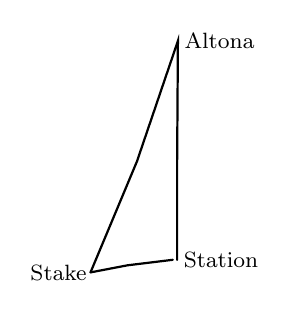
\begin{tikzpicture}[x=1mm,y=1mm,line width=.8pt,line cap=round]
  \coordinate (Pfahl) at (0,0);
  \coordinate (Altona) at (11.1,29.4);
  \coordinate (Standpunkt) at (11.0,1.6);
  \draw (Pfahl) -- (5.9,14.1) -- (Altona) -- (11.0,14.0) -- (Standpunkt);
  \draw (Pfahl) -- (4.7,.9) -- (10.45,1.6);
  \node[font=\footnotesize,anchor=east,inner sep=1pt] at (Pfahl) {Stake};
  \node[font=\footnotesize,anchor=west,inner sep=2pt] at (Altona) {Altona};
  \node[font=\footnotesize,anchor=west,inner sep=2pt] at (Standpunkt) {Station};
 \end{tikzpicture}
\end{minipage}\hfill
\begin{minipage}[t]{.71\linewidth}
 \vspace{0pt}
 \setlength{\parindent}{1.5em}
 \indent I,\quad The angle at Altona between the directions to the stake and to the station.

 II.\quad A small correction for the curvature of the Earth, owing to which the difference between the directions Altona-station and station-Altona is slightly different from \(180^\circ\). The two adjustments can
\end{minipage}\par
\noindent only be computed when the position of the station is already known at least approximately. One may therefore find this position first, leaving those two adjustments aside for the time being. This needs no instruction. You may use the \(\Delta\) Altona, station, Hamburg or Altona, station, Rönneberg, etc., as you please. I only note that computing I requires just the distance from Altona to the station. In the triangle above, 2 sides and one angle are then known. I now find
\[
\raisebox{\baselineskip}{\(\displaystyle
\GaussRightBrace{
\begin{array}{@{}l@{\;=\;}l@{}}
 \log(\text{Altona-station})&4{,}09915\\
 \log(\text{station-stake})&0{,}16643\\
 \text{Angle [at] station}&129^\circ36'58''
\end{array}}
\)}
\begin{array}{@{}l@{\;}c@{\;}r@{}}
 \text{The angle at Altona}&=&18''{,}551\\
 \text{and hence, since at Altona}&&\\
 \text{Azimuth of the stake}&=&13^\circ\,34'\,20''{,}225,\\
 \cline{2-3}
 \text{at the same place}&&\\
 \text{Azimuth of the station}&=&13^\circ\,34'\,1''{,}674.
\end{array}
\]

As to II, I note that this correction requires the approximate coordinates of the station.

If the coordinates of Altona are \(a,b\),\par
and those of the station \(x,y\),\par
the correction is \(=-A(x-a)(y+b)\),\par
\noindent where \(A\) is a quantity that is actually a function of \(x\), or more precisely of \(\frac12(x+a)\), but varies very slowly[*)].
\[
\begin{array}{@{}c@{\quad}l@{\quad}c@{\enspace}c@{\;=\;}l@{}}
 \text{For}&\text{Altona,}&\text{we have}&\log A&1{,}40336-10\\
 \text{»}&\text{Lysabbel}&\text{»}&\text{»}&1{,}40323-10.
\end{array}
\]
\indent The calculation therefore runs as follows.
\[
\begin{array}{@{}r@{\;=\;}r@{\qquad}r@{\;=\;}r@{\enspace}l@{}}
 a&-224495{,}3&b&+16{,}4&\\
 x&-212281{,}4&y&+2963{,}7&\text{(already good coordinates, incidentally)}
\end{array}
\]

\par\smallskip\noindent\rule{4cm}{.4pt}\par
{\footnotesize\noindent\hspace*{\parindent}[*) Cf. pp.~216/217, where \(q\) is written for \(A\). If \(A\) is assumed to be the same for both points, the correction is \(-A(x-a)\dfrac{2b+y}{3}+A(a-x)\dfrac{2y+b}{3}\).]\par}

% Printed 287; principal PDF 294; Google PDF 298.
\par\clearpage
\noindent\null\hfill{\small\textbf{STATION ADJUSTMENTS.}}\hfill\makebox[0pt][r]{\fontsize{13}{16}\selectfont 287}\par\medskip

\[
\begin{array}{@{}r@{\;=\;}r@{\qquad}l@{\enspace}l@{}}
 x-a&+12213{,}9&\log.\,.\,.\,.\,.\,.&4{,}08686\\
 y+b&+2980{,}1&\log.\,.\,.\,.\,.\,.&3{,}47423\\
 \multicolumn{2}{c}{}&\log(-A).\, .&1{,}40336_n-10\\
 \cline{3-4}
 \multicolumn{2}{c}{}&&8{,}96445_n-10.
\end{array}
\]
\[
\begin{array}{@{}r@{\quad}c@{\;}l@{}}
 \text{Number}&=&\qquad-0''{,}092.\\[3pt]
 \text{Azimuth \textls[120]{at} Altona}&=&13^\circ\,34'\,1''{,}674\\
 &&180\\
 \cline{3-3}
 \text{Azimuth \textls[120]{from} Altona}&=&193^\circ\,34'\,1''{,}582.
\end{array}
\]
\indent To orient the table above, a correction of \(-28''{,}394\) is therefore required, giving the following.
\[
\begin{array}{@{}l@{\enspace}r@{\;}r@{\;}l@{}}
 \text{\hbox to 8.7em{Stake\hfil.\hfil.\hfil.\hfil.\hfil.\hfil.\hfil.\hfil.\hfil.}}&63^\circ&57'&4''\\
 \text{\hbox to 8.7em{Neuenfelde\hfil.\hfil.\hfil.\hfil.}}&148&22&31{,}267\\
 \text{\hbox to 8.7em{Altenwerder\hfil.\hfil.\hfil.}}&189&27&10{,}451\\
 \multicolumn{4}{c}{\text{etc.}}
\end{array}
\]

\begin{center}\rule{3cm}{.4pt}\end{center}
\vspace{.8cm}
\begingroup\small
\begin{center}
 REMARKS.
\end{center}

There is no compilation of the final adjustments of station observations whose results were incorporated into the network adjustment. The results of the station adjustments themselves are given in Volume IV, pp.~449 ff., in the »Abrissen der auf den verschiedenen Stationen der Gradmessung, 1821, 1822, 1823, und deren Fortsetzung bis Jever, 1824, 1825, festgelegten Richtungen.« Yet the direction values that \textsc{Gauss} used for the network adjustment, as can be seen from the tabulation by triangle of the observed angles in the next section, still differ slightly from those values. The differences arise from the reductions for the height of the object sighted and for the departure of the geodesic from the vertical section (cf. the letter to \textsc{Olbers} of 14 May 1826 reproduced below). For some directions they must also arise from centering corrections.

The station adjustments for Zeven and Brillit given here, [1] and [2], are provisional and were taken from a notebook in which \textsc{Gauss} had recorded 8 adjustments of station observations in all. In place of the stated constants in the third and fourth normal equations for Zeven, \textsc{Gauss} mistakenly had \(+0{,}346\) and \(-1{,}189\). His solution table consequently differs from the one given above. As the observations progressed, \textsc{Gauss} repeated the adjustments several times (cf. p.~280, at the bottom). Thus the adjustment for the Wilsede station given here, Note [3], was the fourth, which was found in a book of observations and computations for the Hanoverian arc measurement. Its result agrees with the entry in the »Abrissen

% Printed 288; principal PDF 295; Google PDF 299.
\par\clearpage
\noindent\makebox[0pt][l]{\fontsize{13}{16}\selectfont 288}\hfill{\small\textbf{REMARKS.}}\hfill\null\par\medskip

\noindent etc.«, Volume IV, p.~454, if the orientation here is changed by \(-0''{,}665\). If we calculate for Wilsede, according to Art.~13, p.~95, the corrections to the observed directions for the elevation above sea level of the object sighted and for the departure of the geodesic from the vertical section, we obtain \(+0''{,}001\) for the direction to Falkenberg (150,8 m), \(+0''{,}003\) to Elmhorst (90,0 m), \(0''{,}000\) each for the directions to Steinberg (72,3 m), Bottel (52,4 m), Bullerberg (53,3 m), Brüttendorf (49,6 m), and Zeven (44,8 m), \(-0''{,}001\) for the direction to Litberg (65,5 m), \(0''{,}000\) to Hamburg (144,9 m), \(+0''{,}002\) to Lüneburg (99,1 m), \(-0''{,}001\) to Nindorf (116,7 m), \(-0''{,}002\) to Timpenberg (117,1 m), \(-0''{,}003\) to Wulfsode (104,5 m), \(-0''{,}002\) to Breithorn (120,5 m), and \(-0''{,}002\) to Hauselberg (120,4 m). The elevations above sea level in parentheses are taken from one of \textsc{Gauss}'s notebooks. Applying these corrections to the adjustment results gives the values for Wilsede incorporated into the network adjustment.

All the surviving station adjustments are found partly in small books of observations and computations for the arc measurement and partly scattered on loose sheets. At all the principal triangulation points the form of adjustment is as at Zeven or Wilsede, and in a few cases as at Brillit (cf. the letters to \textsc{Olbers} of July 1825, to \textsc{Schumacher} of 14 August 1825, and to \textsc{Bessel} of 29 October 1843).

The measurements were not arranged symmetrically at any principal triangulation point. All angle combinations seem to have been observed only at a few secondary points. One example is provided by the observations on the Windberg, Note [4], by artillery lieutenant F.~\textsc{Hartmann}, one of \textsc{Gauss}'s assistants in the triangulation. (On the original, a single sheet, \textsc{Hartmann} also added, “Incomplete because the mail is leaving. I intend to measure the angle \(7.3\) once more. Perhaps repeating it will also have a favorable effect on the angle \(3.5\).” According to the observation book, however, he did not repeat it.) The measurements on the Windberg were made in June 1830.

The extract from an observation book for the arc measurement point Breithorn, Note [5], shows how \textsc{Gauss} observed.

The following extract from the booklet mentioned earlier, entitled »Geodätischer Calcül nach \textsc{Gauss}« by Prof. \textsc{Goldschmidt}, also describes the procedure used in the Hanoverian triangulation. As already mentioned, \textsc{Goldschmidt} probably helped \textsc{Gauss} with the calculations in the final years of the land survey. In 1834 he took part in the measurements for the detailed survey with Lieutenant \textsc{Gauss}.

»In the triangulation itself one first selects a moderate number of points covering the area to be surveyed in such a way that they command a wide view. One selects only as many of these \textls[120]{principal points} as are needed to determine the so-called points of the second order, which we shall discuss shortly. Their spacing is made as large as the terrain and the power of the telescopes to be used will permit. At \textls[120]{each} of the selected principal triangulation points one sights every visible object whose position is to be determined, but chiefly measures, by multiple repetitions, the angles between the other principal points visible from there. The angles between the selected secondary points and the principal points are measured in the same way.

The principal triangulation points serve to give the whole system a stable framework. One therefore selects only a few of them and sets them as far apart as possible, so as to have fewer intermediate stations at which the errors made could accumulate further and further.

The small number of principal triangulation points selected would, however, make it impossible to determine accurately all the points enclosed by them, even if the terrain allowed us

% Printed 289; principal PDF 296; Google PDF 300.
\par\clearpage
\noindent\null\hfill{\small\textbf{STATION ADJUSTMENTS.}}\hfill\makebox[0pt][r]{\fontsize{13}{16}\selectfont 289}\par\medskip

\noindent to sight every point whose position is to be fixed. Many points would inevitably have to be determined by very acute triangles, in which, as is well known, a very small error in measuring the angles would change the position of the point enormously. This is why a larger number of \textls[120]{secondary points} is also selected.

These are selected so that 1) they suffice to determine \textls[120]{all} the points to be fixed, and 2) \textls[120]{where possible} they can themselves be determined \textls[120]{precisely} from the principal triangulation points. There is no need to insist too strictly on the latter condition, since a point that cannot be determined from principal triangulation points can be determined from secondary points. For the sake of orientation, however, it is always advisable to sight at least one principal triangulation point. From the secondary points, too, one sights \textls[120]{every visible} object to be determined. The principal and secondary points are sighted with multiple repetitions and readings. If need be, the remaining points, which are not stations, are sighted only once.

That is the general outline of the triangulation. A few remarks on the details now follow.\par
\noindent Turning the alidade circle always causes the graduated circle to turn, however slightly. This can produce constant errors, such that if one measures from left to right and always moves the alidade circle to the object along the shorter path, the angles will always come out too small. (In analyzing the measurements that Lieutenant \textsc{Gauss} made in Westphalia in 1833, I found the mean error resulting from this to be about \(1''{,}5\), and in Captain \textsc{Müller}'s measurements, \(3''\).) To compensate for this, \textsc{Gauss} brings the alidade circle into the direction of the second object by the shorter path as often as by the longer one.

\begin{center}
 \textls[120]{Measuring angles from a station.}
\end{center}

We first select a few points whose shape permits precise pointing. For precise results there should probably be at least 4, and to avoid unnecessary work there should be no more than 6. It is best if they are principal points of the system and at the same time divide the horizon into equal parts. There is no need to insist too strictly on these conditions, however. We then measure the angles between pairs of these objects, taking all possible combinations. Next we adjust the values found by the method of least squares. We then compare every other point to be fixed with one of the directions determined in this way. If the point is to be determined more precisely, we use several repetitions, and may even compare it with two of the directions. If these give different results, we apply the method of least squares here as well. We shall now explain how this is done.

We shall illustrate the application of the method of least squares by an example. From the station \textls[120]{Hoheegge}, \textls[120]{Enegerloh} (1), \textls[120]{Dörenberg} (2), \textls[120]{Nonnenstein} (3), and \textls[120]{Hünenburg} (4) were selected as comparison points, and the following angles were measured, each with 20 repetitions.
\[
\begin{array}{@{}r@{\;=\;}r@{\;}r@{\;}l@{}}
 1.2&77^\circ&42'&38''{,}313\\
 1.3&162&40&2{,}500\\
 2.3&84&57&24{,}750\\
 3.4&107&59&41{,}375\\
 4.1&89&20&16{,}438\\
 4.2&167&2&53{,}025.
\end{array}
\]

Now take the azimuths of the 4 points 1, 2, 3, 4, that is, refer them all to one and the same fundamental direction. It is immaterial whether this is actually the meridian, though it is advisable
\par\smallskip\noindent\makebox[0pt][l]{\small IX.}\makebox[.86\linewidth][r]{37}\par

% Printed 290; principal PDF 297; Google PDF 301.
\par\clearpage
\noindent\makebox[0pt][l]{\fontsize{13}{16}\selectfont 290}\hfill{\small\textbf{REMARKS.}}\hfill\null\par\medskip

\noindent to keep this direction fairly close to the meridian so that the correction for orientation will be modest. If necessary, the approximate direction of the meridian can always be obtained with a surveyor's compass (as \textsc{Hartmann} did in the Harz where he knew no azimuth). An approximate value for the azimuth of 1 is \(41^\circ25'0''{,}0\). If all the angles with 1 as one of their sides were measured correctly, the azimuths would be
\[
\begin{array}{@{}r@{\;=\;}r@{\;}r@{\;}l@{}}
 2&119^\circ&7'&38''{,}313\\
 3&204&5&2{,}500\\
 4&312&4&43{,}562.
\end{array}
\]

For example, suppose we replace the computation of 3 from 1 and \(1.3\) with the computation from 2 and \(2.3\). We obtain \(3=2+2.3=204^\circ5'3''{,}063\), which differs from the value given above. We must therefore still apply corrections to 2, 3, 4. The values for 2, 3, 4 are only approximate. To simplify the calculation, we leave out the decimal parts of the arcsecond and include them in the correction. This gives
\[
\begin{array}{@{}r@{\;=\;}r@{\;}r@{\;}r@{\;}l@{}}
 1&41^\circ&25'&0''{,}0&\\
 2&119&7&38{,}0&+x\\
 3&204&5&2{,}0&+y\\
 4&312&4&43{,}0&+z.
\end{array}
\]

Computing the angles from these values gives the following.
\[
\begin{array}{@{}r@{\;=\;}r@{\;}r@{\;}r@{\;}l|r|r@{\;}l@{\;=\;}l@{}}
 \multicolumn{5}{c}{\text{Calc.}}&
 \multicolumn{1}{c}{\text{Obs.}}&
 \multicolumn{3}{c}{\text{Obs.-Calc.}}\\
 1.2&77^\circ&42'&38''{,}0&+x&38''{,}313&-0''{,}313&+x&\varepsilon'\\
 1.3&162&40&2{,}0&+y&2{,}500&-0{,}500&+y&\varepsilon''\\
 2.3&84&57&24{,}0&-x+y&24{,}750&-0{,}750&-x+y&\varepsilon'''\\
 3.4&107&59&41{,}0&-y+z&41{,}375&-0{,}375&-y+z&\varepsilon^{\mathrm{IV}}\\
 4.1&89&20&17{,}0&-z&16{,}438&+0{,}562&-z&\varepsilon^{\mathrm{V}}\\
 4.2&167&2&55{,}0&+x-z&53{,}025&+1{,}975&+x-z&\varepsilon^{\mathrm{VI}}
\end{array}
\raisebox{-.5\baselineskip}{%
 \(\GaussRightBrace{\vphantom{\begin{array}{c}0\\0\\0\\0\\0\\0\end{array}}}\)%
 \enspace\rotatebox[origin=c]{-90}{Error equations.}%
}
\]

Forming the fundamental equations from these by the method of least squares gives
\[
\begin{array}{@{}r@{\;}r@{\;}r@{\;}r@{\;=\;}l@{}}
 +2{,}412&+3x&-y&-z&0\\
 -0{,}875&-x&+3y&-z&0\\
 -2{,}912&-x&-y&+3z&0.
\end{array}
\]

Equations of this form are most easily solved as follows. Adding them gives
\[
 -1{,}375+x+y+z=0,
\]
and adding this equation to each individual fundamental equation gives the following.
\[
\begin{array}{@{}r@{\;}l@{\;=\;}r@{\qquad}c@{\;=\;}l@{}}
 +1{,}037&+4x&0&x&-0{,}259\\
 -2{,}250&+4y&0&y&+0{,}563\\
 -4{,}287&+4z&0&z&+1{,}072.
\end{array}
\]

This simple elimination method can always be used with the symmetric fundamental equations to which this problem leads whenever all combinations of directions have been measured with the same number of repetitions. We thus obtain the adjusted azimuths.

% Printed 291; principal PDF 298; Google PDF 302.
\par\clearpage
\noindent\null\hfill{\small\textbf{STATION ADJUSTMENTS.}}\hfill\makebox[0pt][r]{\fontsize{13}{16}\selectfont 291}\par\medskip

\[
\begin{array}{@{}l@{\quad}r@{\;}r@{\;}r@{\quad}l@{\quad}r@{\quad}r@{\;}r@{\;}r|l@{}}
 \multicolumn{6}{c}{}&\multicolumn{3}{c}{\text{Calc.}}&\multicolumn{1}{c}{\text{Calc.-Obs.}}\\
 1.&41^\circ&25'&0''{,}000&&1.2&77^\circ&42'&37''{,}741&-0''{,}572\\
 2.&119&7&37{,}741&&1.3&162&40&2{,}563&+0{,}063\\
 3.&204&5&2{,}563&&2.3&84&57&24{,}822&+0{,}072\\
 4.&312&4&44{,}072&\text{and hence}&3.4&107&59&41{,}509&+0{,}134\\
 &&&&&4.1&89&20&15{,}928&-0{,}510\\
 &&&&&4.2&167&2&53{,}669&+0{,}644.
\end{array}
\]

If the numbers of repetitions used to measure the angles vary, giving them different weights, each contribution of the error equations for \(\varepsilon',\varepsilon'',\varepsilon''',\ldots\) to the fundamental equations must be multiplied by its weight, that is, by the number proportional to the number of repetitions. To give an example of this case as well, we take the angles measured by [Lieutenant] \textsc{Gauss} at \textls[120]{Neuenkirchen}.

\begin{center}
 1. Dörenberg\qquad 2. Quekenberg\qquad 3. Quackenbrück\qquad 4. Mordkuhlenberg.
\end{center}

He found
\[
\begin{array}{@{}r@{\quad}r@{\;}r@{\;}r@{\quad}c@{\qquad}l@{\quad}r@{\;}r@{\;}r@{\;}l@{}}
 \multicolumn{4}{c}{}&\text{Wt.}&
 \multicolumn{5}{c}{\text{Azimuths}}\\
 1.2&93^\circ&9'&2''{,}875&5&1.&6^\circ&25'&58''{,}000&\quad\text{[*)]}\\
 1.3&147&10&10{,}938&1&2.&99&35&0{,}875&+b\\
 2.3&54&1&4{,}125&5&3.&153&36&5{,}656&+c\\
 3.4&86&21&14{,}875&5&4.&239&57&22{,}453&+d\\
 4.1&126&28&33{,}625&5&&&&&\\[3pt]
 &\multicolumn{3}{c}{\text{Calc.-Obs.}}&\text{Wt.}&&&&&\\
 1.2&&&0''{,}000+b&5&&&&&\\
 1.3&&&-3{,}282+c&1&&&&&\\
 2.3&&&+0{,}656-b+c&5&&&&&\\
 3.4&&&+1{,}922-c+d&5&&&&&\\
 4.1&&&+1{,}922-d&5.&&&&&
\end{array}
\]

Forming the fundamental equations by multiplying the contributions of the error equations above by their respective weights gives
\[
\begin{array}{@{}r@{\;}c@{\;}r@{\;}c@{\;=\;}l@{}}
 -3{,}280&+10b&-5c&*&0\\
 -9{,}612&-5b&+11c&-5d&0\\
 \multicolumn{1}{c@{\;}}{0}&*&-5c&+10d&0,
\end{array}
\]
and \(b,c,d\) are now found by the usual rules, thus improving the azimuth values above.

Once the angles measured between the principal directions have been adjusted in this way, they are used to determine the remaining directions, which, as already stated, are linked to one of the adopted principal directions when sighted. If, for example, a point \(A\) is linked to principal direction 1, whose azimuth we call 1, by measuring the angle \(1.A\), then we have the azimuth of \(A=1+1.A\).

\par\smallskip\noindent\rule{4cm}{.4pt}\par
{\footnotesize\noindent\hspace*{\parindent}[*) In a set of lecture notes on higher geodesy that also contains this example, a correction is likewise assigned to the direction toward 1, so that the sum of the normal equations becomes zero.]\par}
\par\smallskip\noindent\makebox[.86\linewidth][r]{37\textsuperscript{*}}\par
\endgroup
